\begin{frame}{Methodology}{Datasets and Feature Extraction}
  \begin{itemize}
    \item \textbf{NIH Chest X-ray 10k}: 7,500 SAE training / 2,500 validation images; no text or labels.
    \item \textbf{Open-I}: Evaluation pool of 3,666 frontal image--report pairs; Findings + Impression.
    \item \textbf{Features}: Frozen BiomedCLIP ViT-B/16 image encoder; \textbf{512-dimensional embeddings}.
  \end{itemize}
  {\centering
    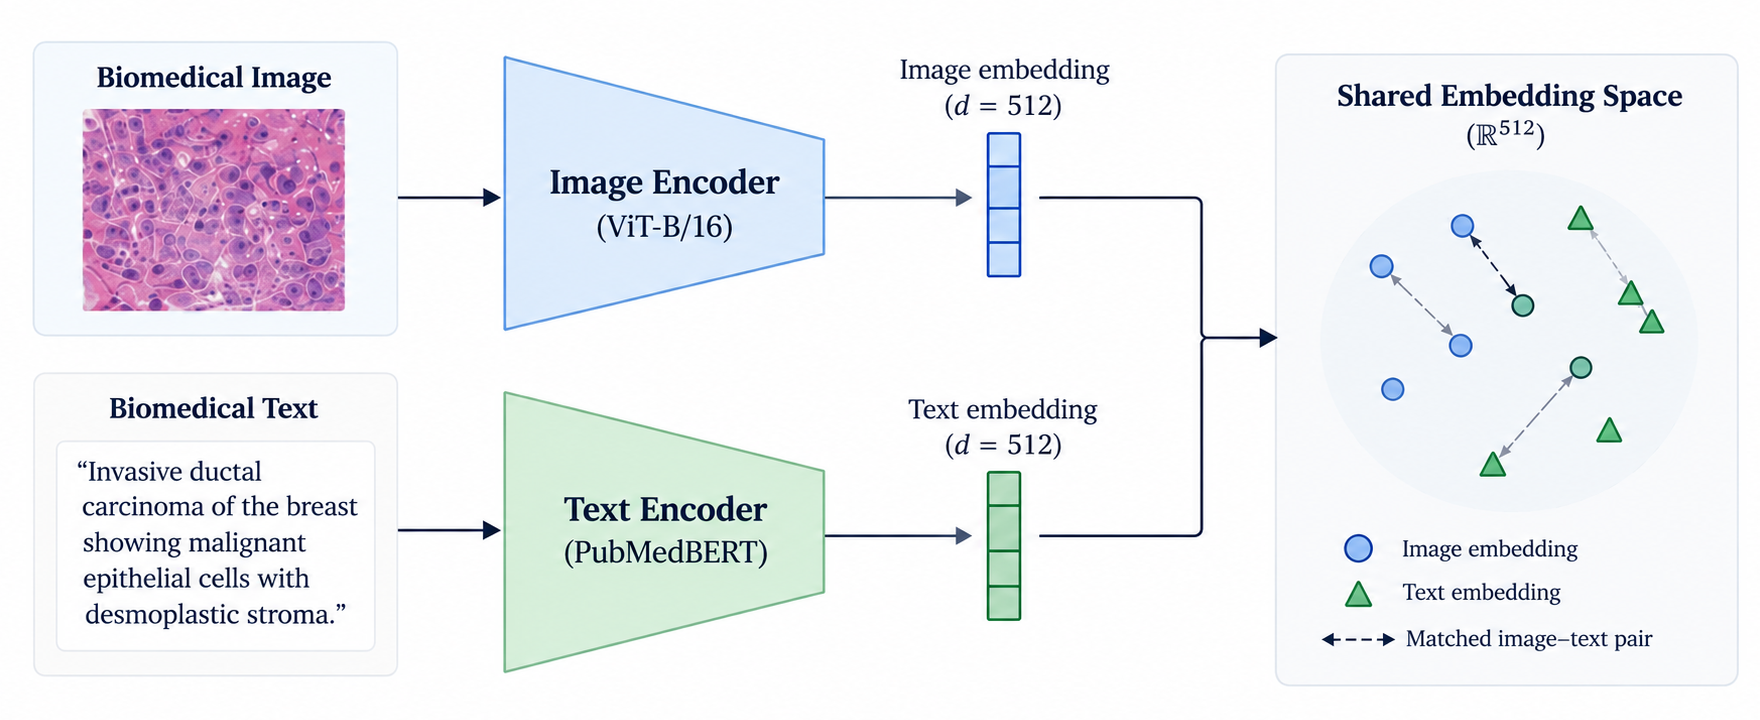
\includegraphics[width=0.60\textwidth,keepaspectratio]{assets/Biomedclip.png}
    \par
    {\footnotesize BiomedCLIP overview\par}
  }

  \note{
  }
\end{frame}


\begin{frame}{Methodology}{Concept Dictionary Construction}
  \begin{itemize}
    \item \textbf{Concept Selection}: 100 parent concepts from cleaned and filtered Open-I Problems metadata, covering anatomy and pathological findings.
    \item \textbf{Expansion}: UMLS provides Concept Unique Identifiers (CUIs) and synonyms from SNOMED CT and MeSH for matched concepts.
    \item \textbf{Phrase Generation}: Gemini 3.1 Flash-Lite generates 5 radiology-style descriptions per concept.
    \item \textbf{Encoding}: BiomedCLIP's PubMedBERT text encoder maps all 998 dictionary entries to L2-normalized, 512-dimensional embeddings in the same space as the images.
  \end{itemize}
  {\Large
  \[
    T \in \mathbb{R}^{998 \times 512}
  \]
  }

  \note{
  }
\end{frame}


\begin{frame}{Methodology}{Sparse Autoencoder Architecture and Training}
  \begin{columns}[c,onlytextwidth]
  \begin{column}{0.66\textwidth}
  \begin{itemize}
    \item \textbf{Architecture}: 512-dimensional input, 1,024 hidden units
    (overcomplete factor of 2), ReLU activations $z$.
    \medskip
    \item \textbf{Objective}: Reconstruction error plus an $L_1$ penalty on activations; $\lambda$ controls the sparsity penalty.
    \[
      \mathcal{L}=\frac{1}{512B}\sum_{i=1}^{B}\|x_i-\hat{x}_i\|_2^2
      +\frac{\lambda}{B}\sum_{i=1}^{B}\|z_i\|_1
    \]
    \item \textbf{Optimization}: Adam, batch size $B=256$. Validation loss guides early stopping and model selection.
  \end{itemize}
  \end{column}
  \begin{column}{0.30\textwidth}
    \centering
    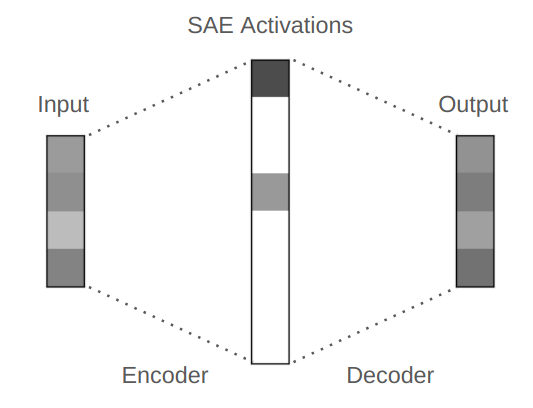
\includegraphics[width=\linewidth,keepaspectratio]{assets/SAE_diagram.png}
    \par\smallskip
    {\footnotesize Illustrative SAE architecture}
  \end{column}
  \end{columns}

  \note{
  }
\end{frame}


\begin{frame}{Methodology}{Concept Assignment and Inference}
  After SAE training, each decoder column represents a learned feature direction
  in the image embedding space.
  \medskip
  \begin{itemize}
    \item \textbf{Naming}: Compare normalized decoder columns $\widetilde{W}_d$ with
    dictionary embeddings $T$. Assign the entry with the highest cosine similarity
    to each feature.
    {
    \[
      S=T\widetilde{W}_d\in\mathbb{R}^{998\times1024}
    \]
    }
    \item \textbf{Inference}: Rank positive SAE activations for each Open-I image.
    Select features from largest to smallest until cumulative activation $>$ \textbf{90\% of the total positive activation}.
    \item \textbf{Output}: Collect the selected features' labels and remove duplicate
    phrases to obtain the predicted concept set.
  \end{itemize}

  \note{
  }
\end{frame}


\begin{frame}{Methodology}{Semantic Evaluation and Validation}
  \begin{itemize}
    \item \textbf{Evaluator}: Frozen MedGemma 1.5 4B receives a concept phrase and
    its reference report, without the image.
    \item \textbf{Verdicts}:
    \begin{itemize}
        \item[\textcolor{green!60!black}{$\checkmark$}] \textbf{Aligned}: Report explicitly supports the concept.
        \item[\textcolor{red}{$\times$}] \textbf{Unaligned}: Report explicitly negates or contradicts the concept.
        \item[\textcolor{orange}{$?$}] \textbf{Uncertain}: Concept is unmentioned, ambiguous, or tentative.
    \end{itemize}
    \item \textbf{Bias Mitigation}: Rotate class--letter mappings across 3 passes;
    select the verdict with the highest average probability.
    \item \textbf{Clustering}: Group parent concepts with hierarchical clustering
    and compare alignment across groups using existing verdicts.
    \item \textbf{Validation}: 25 pairs independently labelled by 3 authors, blinded
    to MedGemma's verdicts. Compare MedGemma and 3 commercial models against majority vote.
  \end{itemize}

  \note{
  }
\end{frame}
